% option draft um zu lange Zeilen anzuzeigen
\documentclass[a4paper,11pt,draft]{article}

\usepackage[inner=3cm,outer=3cm]{geometry}
\usepackage[english]{babel}
\usepackage[utf8]{inputenc}
% linux libertine for normal text
\usepackage{libertine}
\usepackage{libertinust1math}
% inconsolate as teletype font
\usepackage{inconsolata}
\usepackage[T1]{fontenc}
\usepackage{color}
\usepackage{graphicx}
\usepackage{wrapfig}
\usepackage{amsmath}
\usepackage{amssymb}
\usepackage{subcaption}
\usepackage{pmboxdraw}
\usepackage{lipsum}
\usepackage[export]{adjustbox}
\usepackage{csquotes}
\usepackage{tabularx}
\usepackage[sort]{natbib}
\usepackage[toc,nonumberlist]{glossaries}
\usepackage{makecell}
\usepackage[absolute,overlay]{textpos}
\usepackage{microtype}
\usepackage[linesnumbered,ruled]{algorithm2e}

% setup of siunitx
\usepackage[binary-units=true]{siunitx}
\DeclareSIUnit{\bits}{bits}
\DeclareSIUnit{\cycle}{cycle}
\DeclareSIUnit{\cycles}{cycles}
\sisetup{
  list-final-separator = {, and },
  per-mode=symbol
}

% tikz
\usepackage{tikz}
\usepackage{tikz-uml}
\usetikzlibrary{arrows,automata,positioning}
\usetikzlibrary{shapes.geometric}
\usetikzlibrary{shapes.multipart}
\usetikzlibrary{arrows.meta}
\usetikzlibrary{calc}
\usetikzlibrary{intersections}
\usetikzlibrary{patterns}

% tikz setup
\usepackage{environ}
\makeatletter
\newsavebox{\measure@tikzpicture}
\NewEnviron{scaletikzpicturetowidth}[1]{%
  \def\tikz@width{#1}%
  \def\tikzscale{1}\begin{lrbox}{\measure@tikzpicture}%
  \BODY
  \end{lrbox}%
  \pgfmathparse{#1/\wd\measure@tikzpicture}%
  \edef\tikzscale{\pgfmathresult}%
  \BODY
}

\makeatother
\tikzstyle{thick arrow}=[-{Latex[length=2mm]}]

% hyperlinks
\usepackage[hyphens]{url}
\usepackage{hyperref}
\hypersetup{
  pdfauthor   = {Nils Asmussen},
  pdftitle    = {DTU Specification},
  pdfborder   = {0 0 0 [0 0]},
  colorlinks  = false
}

% listings
\usepackage{listings}
\lstset{basicstyle=\small\ttfamily,breaklines=true}
\lstdefinestyle{myc++}{
  language=C++,
  morekeywords={size_t,ssize_t}
}

% ignore page group warnings
\pdfsuppresswarningpagegroup=1

% redefine some names
\addto\extrasenglish{%
  \renewcommand{\chapterautorefname}{Chapter}%
  \renewcommand{\sectionautorefname}{Section}%
  \renewcommand{\subsectionautorefname}{Section}%
  \renewcommand{\subsubsectionautorefname}{Section}%
}

% for smart references
\newcommand{\rref}[2][]{\autoref{#2}}

% names
\newcommand{\myos}{$\text{M}^\mathbf{3}$}
\newcommand{\myfs}{$\text{M}^\mathbf{3}$FS}

% TODOs
\newcommand{\todo}[1]{\fbox{\bfseries\sffamily\scriptsize\color{red}TODO: #1}}

\title{DTU Specification}
\author{Nils Asmussen}
\date{\today}

\begin{document}

\maketitle

\section{Overview}

\begin{figure}[h]
  \center
  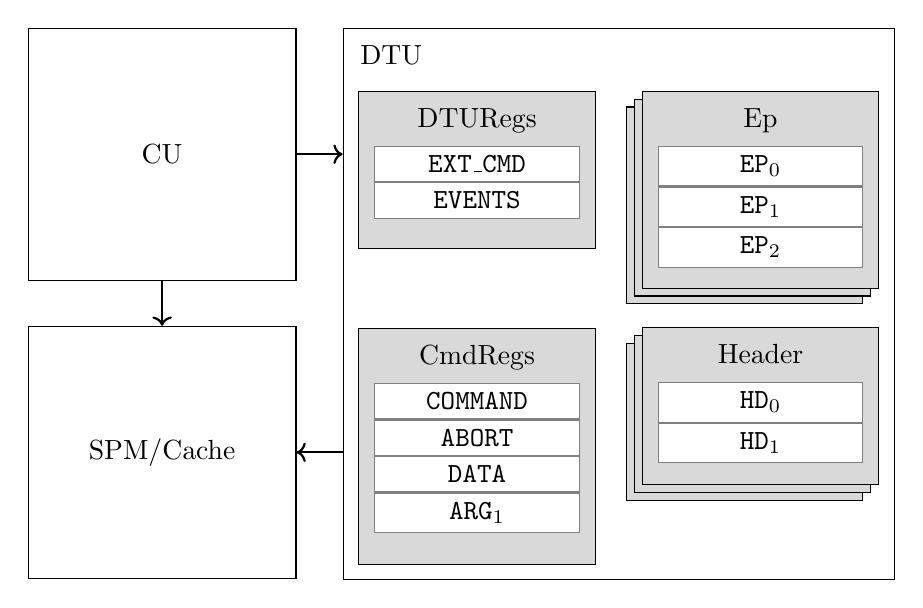
\begin{tikzpicture}[
      dtureg/.style={draw=gray,fill=white,minimum width=2.6cm},
      regtbl/.style={draw=black,fill=gray!30,minimum width=3cm}
    ]

    \node[draw=black,minimum width=7cm,minimum height=7cm,anchor=north west] (dtu) at(4,0) {};
    \node[draw=black,minimum width=3.4cm,minimum height=3.2cm,anchor=north west] (cu) at (0,0) {CU};
    \node[draw=black,minimum width=3.4cm,minimum height=3.2cm,anchor=south west] (mem) at (0,-7) {SPM/Cache};

    \node[below right=.1cm and .1cm of dtu.north west] {DTU};

    \node[
      regtbl,below right=.8cm and .2cm of dtu.north west,minimum height=2cm
    ] (dturegs) {};
    \node[below=.1cm of dturegs.north] {DTURegs};
    \node[dtureg,below=.7cm of dturegs.north] (dtureg0) {\texttt{EXT\_CMD}};
    \node[dtureg,below=0cm of dtureg0]        (dtureg1) {\texttt{EVENTS}};

    \node[
      regtbl,below=1cm of dturegs.south,minimum height=3cm
    ] (cmdregs) {};
    \node[below=.1cm of cmdregs.north] {CmdRegs};
    \node[dtureg,below=.7cm of cmdregs.north] (cmdreg0) {\texttt{COMMAND}};
    \node[dtureg,below=0cm of cmdreg0]        (cmdreg1) {\texttt{ABORT}};
    \node[dtureg,below=0cm of cmdreg1]        (cmdreg2) {\texttt{DATA}};
    \node[dtureg,below=0cm of cmdreg2]        (cmdreg3) {\texttt{ARG$_1$}};

    \node[
      regtbl,below left=1cm and .4cm of dtu.north east,minimum height=2.5cm
    ] {};
    \node[
      regtbl,below left=.9cm and .3cm of dtu.north east,minimum height=2.5cm
    ] {};
    \node[
      regtbl,below left=.8cm and .2cm of dtu.north east,minimum height=2.5cm
    ] (epregs) {};
    \node[below=.1cm of epregs.north] {Ep};
    \node[dtureg,below=.7cm of epregs.north] (epreg0) {\texttt{EP$_0$}};
    \node[dtureg,below=0cm of epreg0]        (epreg1) {\texttt{EP$_1$}};
    \node[dtureg,below=0cm of epreg1]        (epreg2) {\texttt{EP$_2$}};

    \node[
      regtbl,below left=4cm and .4cm of dtu.north east,minimum height=2cm
    ] {};
    \node[
      regtbl,below left=3.9cm and .3cm of dtu.north east,minimum height=2cm
    ] {};
    \node[
      regtbl,below left=3.8cm and .2cm of dtu.north east,minimum height=2cm
    ] (hdregs) {};
    \node[below=.1cm of hdregs.north] {Header};
    \node[dtureg,below=.7cm of hdregs.north] (hdreg0) {\texttt{HD$_0$}};
    \node[dtureg,below=0cm of hdreg0]        (hdreg1) {\texttt{HD$_1$}};

    \path
      let \p1=(cu.east), \p2=(dtu.west) in
      [draw=black,thick,->] (cu.east) -- (\x2,\y1);
    \path[draw=black,thick,->] (cu) -- (mem);
    \path
      let \p1=(mem.east), \p2=(dtu.west) in
      [draw=black,thick,<-] (mem.east) -- (\x2,\y1);
  \end{tikzpicture}
  \caption{Overview of the DTU's registers and its connections to other components.}
  \label{fig:overview}
\end{figure}

As shown in \rref{fig:overview}, the compute unit~(CU) is connected to the data transfer unit~(DTU)
and can access the DTU's registers via memory mapped input/output (MMIO). Additionally, the CU is
connected to the local memory. The DTU is also connected to the local memory to, for example, access
messages. These components are not necessarily arranged in this way. For example, the DTU might
interpose itself between the CU and local memory.

\section{MMIO region}

The MMIO region of the DTU is defined as follows:

\vspace{2ex}
\noindent
\begin{tabular}{ p{3cm} | c | c | l }
  \textbf{Address} & \textbf{Register} & \textbf{Group} & \textbf{Description} \\
  \hline
  \texttt{0xF000\_0000} & \texttt{EXT\_CMD} & DtuRegs & Triggers external commands \\
  \hline
  \texttt{0xF000\_0008} & \texttt{EVENTS} & DtuRegs & Contains outstanding events \\
  \hline
  \texttt{0xF000\_0010} & \texttt{COMMAND} & CmdRegs & Triggers internal commands \\
  \hline
  \texttt{0xF000\_0018} & \texttt{ABORT} & CmdRegs & Aborts internal commands \\
  \hline
  \texttt{0xF000\_0020} & \texttt{DATA} & CmdRegs & Specifies the data for commands \\
  \hline
  \texttt{0xF000\_0028} & \texttt{ARG$_1$} & CmdRegs & Additional argument for commands \\
  \hline
  \texttt{0xF000\_0030} & \texttt{EP$_{00}$} & EpRegs & First register of EP$_0$ \\
  \texttt{0xF000\_0038} & \texttt{EP$_{01}$} & EpRegs & Second register of EP$_0$ \\
  \texttt{0xF000\_0040} & \texttt{EP$_{02}$} & EpRegs & Third register of EP$_0$ \\
  \hline
  \texttt{0xF000\_0048} & \texttt{EP$_{10}$} & EpRegs & First register of EP$_1$ \\
  \texttt{0xF000\_0050} & \texttt{EP$_{11}$} & EpRegs & Second register of EP$_1$ \\
  \texttt{0xF000\_0058} & \texttt{EP$_{12}$} & EpRegs & Third register of EP$_1$ \\
  \hline
  \multicolumn{4}{c}{\dots} \\
  \hline
  \texttt{0xF000\_0100} & \texttt{EP$_{n0}$} & EpRegs & First register of EP$_{n}$ \\
  \texttt{0xF000\_0108} & \texttt{EP$_{n1}$} & EpRegs & Second register of EP$_{n}$ \\
  \texttt{0xF000\_0110} & \texttt{EP$_{n2}$} & EpRegs & Third register of EP$_{n}$ \\
  \hline
  \texttt{0xF000\_0118} & \texttt{HD$_{00}$} & Header & First register of HD$_0$ \\
  \texttt{0xF000\_0120} & \texttt{HD$_{01}$} & Header & Second register of HD$_0$ \\
  \texttt{0xF000\_0128} & \texttt{HD$_{02}$} & Header & Third register of HD$_0$ \\
  \hline
  \texttt{0xF000\_0130} & \texttt{HD$_{10}$} & Header & First register of HD$_1$ \\
  \texttt{0xF000\_0138} & \texttt{HD$_{11}$} & Header & Second register of HD$_1$ \\
  \texttt{0xF000\_0140} & \texttt{HD$_{12}$} & Header & Third register of HD$_1$ \\
  \hline
  \multicolumn{4}{c}{\dots} \\
  \hline
  \texttt{0xF000\_0200} & \texttt{HD$_{n0}$} & Header & First register of HD$_{n}$ \\
  \texttt{0xF000\_0208} & \texttt{HD$_{n1}$} & Header & Second register of HD$_{n}$ \\
  \texttt{0xF000\_0210} & \texttt{HD$_{n2}$} & Header & Third register of HD$_{n}$ \\
\end{tabular}

\section{Endpoints}

The DTU has a number of \emph{endpoints}~(EPs) to establish communication channels, which can be
configured to three different EP types: \emph{send EPs} and \emph{receive EPs} are used for message
passing, whereas \emph{memory EPs} are used for RDMA-like memory access. Each EP is represented by a
DTU register and can be configured (at runtime) to one of these EP types. Each EP consists of 192
bits, starting with 3 bits for the endpoint type and 189 bits, whose meaning depends on the EP type.

\begin{tabular}{ c c }
  Memory EP: &
  \begin{scaletikzpicturetowidth}{0.75\linewidth}
    \begin{tikzpicture}[
      baseline=8ex,scale=\tikzscale,
      reg/.style={fill=gray!20,draw=black},
      undef/.style={fill=gray!20,draw=black,pattern=north east lines, pattern color=black}
    ]
    \path[reg] (0,0) rectangle (3,3) node[midway] {T};
    \path[reg] (3,0) rectangle (64,3) node[midway] {region size};
    \path[reg] (0,3) rectangle (64,6) node[midway] {region base address};
    \path[undef] (0,6) rectangle (20,9) node[midway] {};
    \path[reg] (20,6) rectangle (52,9) node[midway] {VPE ID};
    \path[reg] (52,6) rectangle (60,9) node[midway] {PE ID};
    \path[reg] (60,6) rectangle (64,9) node[midway] {rw};

    \node[anchor=north west,xshift=-3pt] at (0,0)  {63};
    \node[anchor=north east,xshift=3pt]  at (64,0) {0};
    \end{tikzpicture}
  \end{scaletikzpicturetowidth}
  \\
  \\
  Send EP: &
  \begin{scaletikzpicturetowidth}{0.75\linewidth}
    \begin{tikzpicture}[
      baseline=8ex,scale=\tikzscale,
      reg/.style={fill=gray!20,draw=black},
      undef/.style={fill=gray!20,draw=black,pattern=north east lines, pattern color=black}
    ]
    \path[reg] (0,0) rectangle (3,3) node[midway] {T};
    \path[undef] (3,0) rectangle (16,3) node[midway] {};
    \path[reg] (16,0) rectangle (48,3) node[midway] {VPE ID};
    \path[reg] (48,0) rectangle (64,3) node[midway] {max. msg size};
    \path[undef] (0,3) rectangle (16,6) node[midway] {};
    \path[reg] (16,3) rectangle (24,6) node[midway] {PE ID};
    \path[reg] (24,3) rectangle (32,6) node[midway] {EP ID};
    \path[reg] (32,3) rectangle (48,6) node[midway] {max. credits};
    \path[reg] (48,3) rectangle (64,6) node[midway] {cur. credits};
    \path[reg] (0,6) rectangle (64,9) node[midway] {label};

    \node[anchor=north west,xshift=-3pt] at (0,0)  {63};
    \node[anchor=north east,xshift=3pt]  at (64,0) {0};
    \end{tikzpicture}
  \end{scaletikzpicturetowidth}
  \\
  \\
  Receive EP: &
  \begin{scaletikzpicturetowidth}{0.75\linewidth}
    \begin{tikzpicture}[
      baseline=8ex,scale=\tikzscale,
      reg/.style={fill=gray!20,draw=black},
      undef/.style={fill=gray!20,draw=black,pattern=north east lines, pattern color=black}
    ]
    \path[reg] (0,0) rectangle (3,3) node[midway] {T};
    \path[undef] (3,0) rectangle (4,3) node[midway] {};
    \path[reg] (4,0) rectangle (10,3) node[midway] {rpos};
    \path[reg] (10,0) rectangle (16,3) node[midway] {wpos};
    \path[reg] (16,0) rectangle (32,3) node[midway] {max. msg. size};
    \path[reg] (32,0) rectangle (38,3) node[midway] {size};
    \path[reg] (38,0) rectangle (58,3) node[midway] {header};
    \path[reg] (58,0) rectangle (64,3) node[midway] {\#msgs};
    \path[reg] (0,3) rectangle (64,6) node[midway] {buffer address};
    \path[reg] (0,6) rectangle (32,9) node[midway] {unread mask};
    \path[reg] (32,6) rectangle (64,9) node[midway] {occupied mask};

    \node[anchor=north west,xshift=-3pt] at (0,0)  {63};
    \node[anchor=north east,xshift=3pt]  at (64,0) {0};
    \end{tikzpicture}
  \end{scaletikzpicturetowidth}
\end{tabular}

\subsection{Memory EP}

\begin{description}
  \item[VPE ID and PE ID:] the destination PE and VPE ID
  \item[rw:] the permission bits (read = 1, write = 2)
  \item[region:] the base address and size of the region at the destination
\end{description}

\subsection{Send EP}

\begin{description}
  \item[Label:] the label the DTU puts into the header of each sent message
  \item[VPE, PE, EP:] the IDs of the destination VPE, PE, and receive EP
  \item[max. credits:] the initially received (=max) credits
  \item[cur. credits:] the currently owned credits
  \item[max. msg size:] the maximum message size supported by the receiver
\end{description}

\subsection{Receive EP}

\begin{description}
  \item[unread mask:] a bitmask with the unread (not yet fetched) messages in the buffer
  \item[occupied mask:] a bitmask with the occupied slots in the buffer
  \item[buffer address:] the address of the receive buffer in local memory
  \item[rpos:] the read position (for message fetches) within the receive buffer
  \item[wpos:] the write position (for message receptions) within the receive buffer
  \item[max. msg. size:] the maximum message size that fits in a slot
  \item[size:] the number of slots in the receive buffer
  \item[header:] the offset of the headers for this receive buffer in the header table
  \item[\#msgs:] the number of unread messages
\end{description}

\section{Commands}

The CU can use the DTU's endpoints via \emph{internal commands}. The command registers are used to
pass input arguments for a command to the DTU, start a command, and wait until the command is
finished. The following command registers are used:

\vspace{2ex}
\begin{tabular}{ c c }
  \texttt{COMMAND}: &
  \begin{scaletikzpicturetowidth}{0.75\linewidth}
    \begin{tikzpicture}[
      baseline=1ex,scale=\tikzscale,
      reg/.style={fill=gray!20,draw=black},
      undef/.style={fill=gray!20,draw=black,pattern=north east lines, pattern color=black}
    ]
    \path[reg] (0,0) rectangle (48,3) node[midway] {arg$_0$};
    \path[reg] (48,0) rectangle (51,3) node[midway] {err};
    \path[undef] (51,0) rectangle (52,3) node[midway] {};
    \path[reg] (52,0) rectangle (60,3) node[midway] {EP ID};
    \path[reg] (60,0) rectangle (64,3) node[midway] {op};

    \node[anchor=north west,xshift=-3pt] at (0,0)  {63};
    \node[anchor=north east,xshift=3pt]  at (64,0) {0};
    \end{tikzpicture}
  \end{scaletikzpicturetowidth}
  \\
  \\
  \texttt{DATA}: &
  \begin{scaletikzpicturetowidth}{0.75\linewidth}
    \begin{tikzpicture}[
      baseline=1ex,scale=\tikzscale,
      reg/.style={fill=gray!20,draw=black},
      undef/.style={fill=gray!20,draw=black,pattern=north east lines, pattern color=black}
    ]
    \path[reg] (0,0) rectangle (16,3) node[midway] {size};
    \path[reg] (16,0) rectangle (64,3) node[midway] {address};

    \node[anchor=north west,xshift=-3pt] at (0,0)  {63};
    \node[anchor=north east,xshift=3pt]  at (64,0) {0};
    \end{tikzpicture}
  \end{scaletikzpicturetowidth}
\end{tabular}
\vspace{2ex}

\noindent A write to the \texttt{COMMAND} register starts the command with opcode
\texttt{COMMAND.op}. The meaning of the three argument registers depends on the opcode.

\subsection{\texttt{SEND}}

\begin{algorithm}
    $ep \gets$ read\_ep(COMMAND.ep)\;
    \uIf{ep.T == invalid}{exit(COMMAND.err = INV\_EP)}
    \uIf{ep.cur\_crd != UNLIMITED}{
      \uIf{ep.cur\_crd < ep.max\_msg\_size}{exit(COMMAND.err = NO\_CREDITS)}
      ep.cur\_crd -= ep.max\_msg\_size\;
    }
    \BlankLine
    $reply\_ep \gets COMMAND$_0$\;
    $reply\_label \gets ARG$_1$\;
    $header \gets$ \{ ep.label, DATA.size, reply\_label, ownPE, COMMAND.ep, reply\_ep \}\;
    $payload \gets$ read\_mem(DATA.address, DATA.size)\;
    send\_msg(header | payload, ep.PE, ep.EP)\;
    \BlankLine
    COMMAND.op = IDLE\;
 \caption{The DTU's \texttt{SEND} command.}
\end{algorithm}

\end{document}
